\documentclass[10pt]{beamer}
\usepackage{Format/beamerthemeFeather}
% \usepackage{algorithm,algorithmic}

% \usepackage[utf8]{inputenc}
% \usepackage[english]{babel}
% \usepackage[T1]{fontenc}
% \usepackage{helvet}
% \usepackage{subfigure}
% \usepackage{varwidth,xcolor}
% \usepackage[justification=centering]{caption}

\usepackage[]{algorithm2e}
\usepackage{amsmath}
\usepackage{amsfonts}
\usepackage{amssymb}
\usepackage[english]{babel}
\usepackage{caption}
\usepackage{float}
\usepackage{graphicx}
\usepackage[utf8x]{inputenc}
\usepackage{mathtools}
\usepackage{subfig}
\usepackage{url}
\usepackage{multicol}
\usepackage{threeparttable}
\usepackage{array}
\usepackage{mathtools}
\usepackage{babel}
\usepackage{color}
\usepackage{multirow}

\definecolor{orange}{RGB}{255,127,0}
\DeclarePairedDelimiter{\abs}{\lvert}{\rvert}

%%% Commands
% colored hyperlinks
\newcommand{\chref}[2]{
  \href{#1}{{\usebeamercolor[bg]{Feather}#2}}}
 

%%% Title
\title[LCIS]{An Implementation:\\ Laplacian Coordinates for Image Segmentation Method}
\subtitle[]{\textbf{Software engineering}}
\author[Paola~Ardon, Sepehr~MohaimenianPour, \`Eric~Pairet]{Paola~Ardon$^1$, Sepehr~MohaimenianPour$^2$, \`Eric~Pairet$^3$
		\vspace{0.2cm} \\
        $^1\,$ \textit{ardonp@hotmail.com} \\
        $^2\,$ \textit{Voidminded@gmail.com} \\
        $^3\,$ \textit{ericpairet@gmail.com}}
\date{January 11, 2016}


%%% Document
\begin{document}

%%%% %%%% %%%% %%%% %%%% %%%% %%%% %%%% %%%% %%%% 
%%%% %%%% %%%% %%%% %%%% %%%% %%%% %%%% %%%% %%%% 
{\1
 \begin{frame}[plain,noframenumbering] 
  \titlepage
\end{frame}} 

%%%% %%%% %%%% %%%% %%%% %%%% %%%% %%%% %%%% %%%% 
%%%% %%%% %%%% %%%% %%%% %%%% %%%% %%%% %%%% %%%% 
\begin{frame}{Content}{}
\begin{multicols}{2}
  \tableofcontents
\end{multicols}
\end{frame} 
 
%%%% %%%% %%%% %%%% %%%% %%%% %%%% %%%% %%%% %%%% 
%%%% %%%% %%%% %%%% %%%% %%%% %%%% %%%% %%%% %%%% 
\section{Introduction}
\subsection{Problem statement}
\begin{frame}{Introduction}{Problem statement}
	Problem Statement:
      \begin{itemize}
        \item Image segmentation
        \item Seeded segmentation
         \item Why Laplacian Coordinates method?
         \end{itemize}
	
   \vspace{0.5cm}
   Objective:
       \begin{itemize}
         \item ``Given a color image and some manually annotated pixels, provide \\a segmentation of the image in 2 regions using the Laplacian Coordinates for Seeded Image Segmentation algorithm"
        \end{itemize}
    
\end{frame}
%%%%%%%%%%%%%%%%%%%%%%%%%%%%%%%%%%%%%%%%%%%
\subsection{Background}
\begin{frame}{Introduction}{Background}
 Basic concepts:
\begin{itemize}
   
     \item Energy equation:
{     \footnotesize
        \begin{equation}
         E(x) = k_1 \sum_{i \in B} {||x_i-x_B||}^2_2 + k_2\sum_{i \in F} {||x_i-x_F||}^2_2 + k_3\sum_{i \in V} {\abs{\abs{d_i x_i-\sum_{j \in N(i)} { w_{ij} x_{ij}}}}_2^2}
    \end{equation}
   }
        \item Weight equation:
      \begin{equation}
      w_{ij} = e^{-\frac{\beta{||I_i - I_j||}^2 _{\infty}} {\sigma}}
  		\end{equation}

	\item Valency equation:
        
        \begin{equation}
    d_{i} = \sum_{\substack{j\in N_{i}}} w_{ij}
    	\end{equation}

 	\item Linear system:    
       \begin{equation}
       (I_{s} + L^{2})x = b
       \end{equation}
              
\end{itemize}
\end{frame}
%%%%%%%%%%%%%%%%%%%%%%%%%%%%%%%%%%%%%%%%%%%
\subsection{Implementation approach}
\begin{frame}{Introduction}{Implementation approach}
\begin{figure}
  \centering
  \subfloat[][Qt.]{
\includegraphics[width=0.5in]{figures/qt.JPG}}
  ~
  \subfloat[][Eigen \& OpenCV]{
\includegraphics[width=1.5in]{figures/eigenopencv.JPG}}

  ~
  \subfloat[][Gtest]{
\includegraphics[width=1in]{figures/gtest.JPG}}
  ~
  \subfloat[][CMake]{
\includegraphics[width=1in]{figures/cmake.JPG}}
  
  \subfloat[][Doxygen]{
\includegraphics[width=1.5in]{figures/doxygen.JPG}}
  \caption{Tools used for the implementation.}

\end{figure}


\end{frame}

%%%%%%%%%%%%%%%%%%%%%%%%%%%%%%%%%%%%%%%%%%%
%%%
%%%
%%%%%%%%%%%%%%%%%%%%%%%%%%%%%%%%%%%%%%%%%%%
\section{Project management}
\subsection{Timing}
\begin{frame}{Project management}{Gantt chart}
At the very beginning and taking advantage of the preliminary study of the paper, we programmed a schedule in order to achieve the completeness of the project
    \begin{figure}
  \centering
  \subfloat{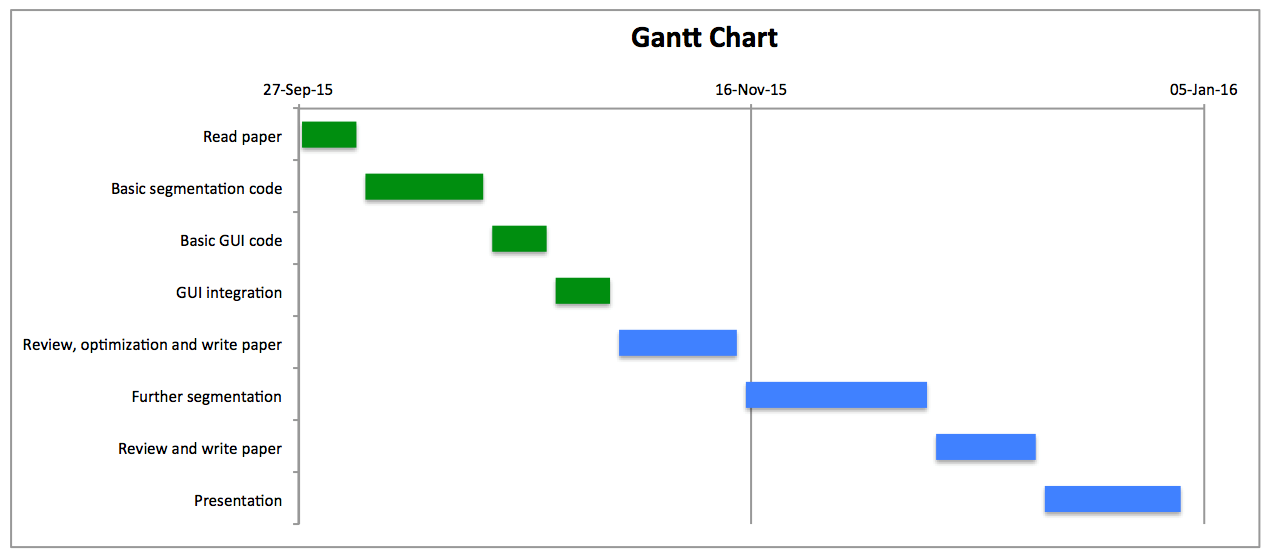
\includegraphics[width=4in]{figures/GANTT.png}}
  \caption{Gantt chart.}
  \end{figure}

\end{frame}
%%%%%%%%%%%%%%%%%%%%%%%%%%%%%%%%%%%%%%%%%%%
\begin{frame} {Project management}{Tasks table}
\begin{minipage}{\textwidth}
  \begin{minipage}[b]{0.42\textwidth}
    \centering
\tiny{
\begin{table}[H]
  \renewcommand{\arraystretch}{1.5}
  \caption{Expected timing for the realization of the project.}
  \begin{center}
    \begin{tabular}{| >{\centering\arraybackslash\bfseries}m{0.36in} | >{\centering\arraybackslash}m{0.26in} | >{\centering\arraybackslash}m{0.26in} | >{\centering\arraybackslash}m{0.24in} |}
    \hline
    Task name & \textbf{Start} & \textbf{End} & \textbf{Duration} (days)\\
    \hline
     Read paper & 28/09/15 & 04/10/15 & 7 \\\hline
    Basic segmentation code & 05/10/15 & 18/10/15 & 14 \\\hline
    Basic GUI code & 19/10/15 & 25/10/15 & 7 \\\hline
    GUI integration & 26/11/15 & 01/11/15 & 7 \\\hline
    Review, optimization and write paper & 02/11/15 & 15/11/15 & 14 \\\hline
    Further segmentation & 16/11/15 & 06/12/15 & 21 \\\hline
    Review and write paper & 07/12/15 & 18/12/15 & 12 \\\hline
    Presentation & 19/12/15 & 03/01/16 & 16 \\
    \hline
    \end{tabular}
  \end{center}
\label{tb:gantt}
\end{table}
}
\end{minipage}
  \hfill
  \begin{minipage}[b]{0.42\textwidth}
    \tiny{
\begin{table}[H]
  \centering
  \renewcommand{\arraystretch}{1.5}
  \caption{Final scheduling of the project.}
  \begin{center}
    \begin{tabular}{| >{\centering\arraybackslash\bfseries}m{0.36in} | >{\centering\arraybackslash}m{0.26in} | >{\centering\arraybackslash}m{0.26in} | >{\centering\arraybackslash}m{0.24in} |}
    \hline
    Task name & \textbf{Start} & \textbf{End} & \textbf{Duration} (days)\\
    \hline
    Read paper & 28/09/15 & 08/10/15 & {\color{orange}11} \\\hline
    Basic segmentation code & 09/10/15 & 18/10/15 & {\color{orange}10} \\\hline
    Basic GUI code & 19/10/15 & 25/10/15 & 7 \\\hline
    GUI integration & 26/11/15 & 03/11/15 & 9 \\\hline
    Review, optimization and write paper & 04/11/15 & 10/11/15 & {\color{orange}7} \\\hline
    Further segmentation & 11/11/15 & 27/12/15 & {\color{orange}47} \\\hline
    Review and write paper & 28/12/15 & 10/01/16 & 14 \\\hline
    Presentation & 28/01/16 & 10/01/16 & 14 \\
    \hline
    \end{tabular}
  \end{center}
\label{tb:gantt2}
\end{table}
}
\end{minipage}
  \end{minipage}

\end{frame}
%%%%%%%%%%%%%%%%%%%%%%%%%%%%%%%%%%%%%%%%%%%
%%%%%%%%%%%%%%%%%%%%%%%%%%%%%%%%%%%%%%%%%%%
\subsection{Tools}
\begin{frame}{Project management}{Tools}

\begin{figure}
  \centering
  \subfloat[][Github]{
\includegraphics[width=1.4in]{figures/github.JPG}}
  ~
  \subfloat[][Trello]{
\includegraphics[width=1.4in]{figures/trello.JPG}}
  ~
   \subfloat[][Overleaf]{
\includegraphics[width=1.4in]{figures/overleaf.png}}
   \caption{Tools used for the project management.}
\end{figure}

\end{frame}
%%%%%%%%%%%%%%%%%%%%%%%%%%%%%%%%%%%%%%%%%%%
%%%
%%%

%%%%%%%%%%%%%%%%%%%%%%%%%%%%%%%%%%%%%%%%%%%%%
\section{System implementation}
\subsection{Basis}
\begin{frame}{System implementation}{Basis}
\begin{figure}
  \centering
  \subfloat{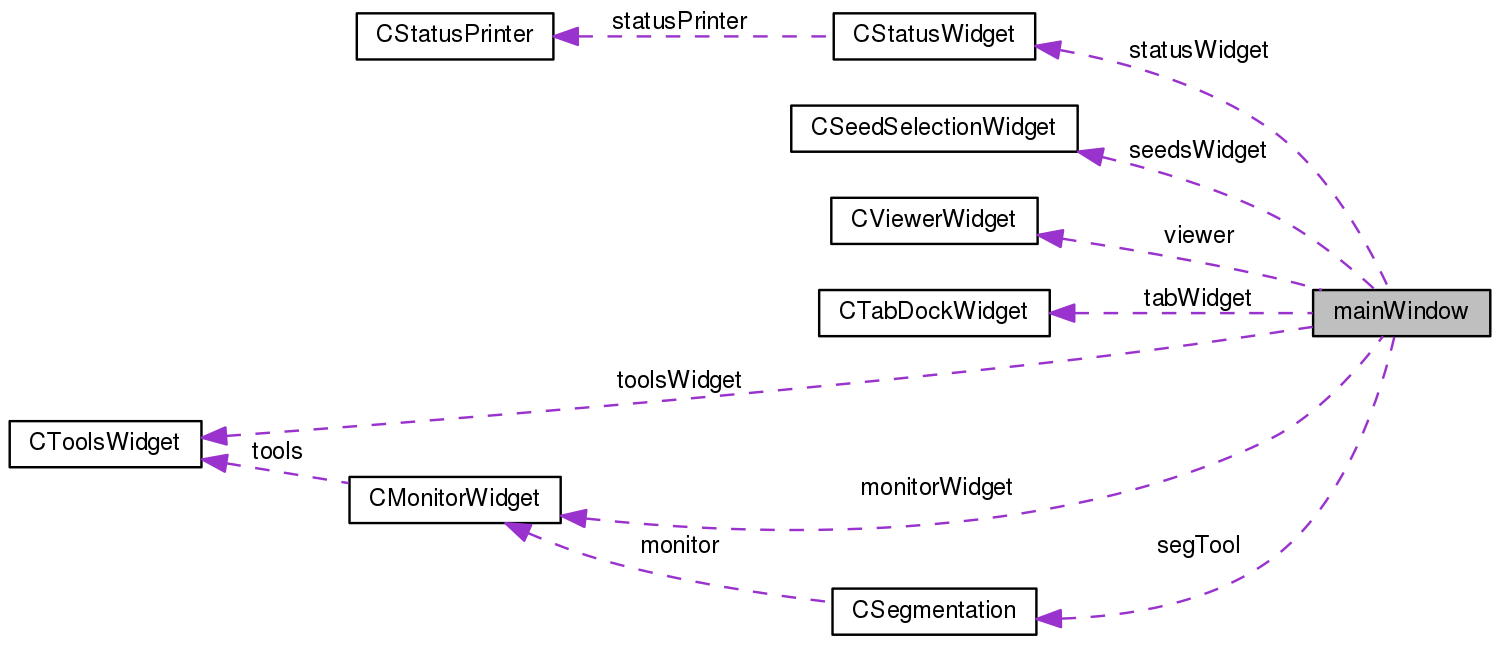
\includegraphics[width=4.5in]{figures/overall.png}}
  \caption{System diagram}
  \end{figure}
\end{frame}

%%%%%%%%%%%%%%%%%%%%%%%%%%%%%%%%%%%%%%%%%%%
\begin{frame}{System implementation}{Basis}
The previously explained algorithm is implemented in two parts:
  \begin{itemize}
      \item Segmentation code
      \item Graphical User Interface (GUI)
  \end{itemize}
  \vspace{0.3in}
Using the following methods in implementation:
\begin{itemize}
	\item Multi-threading
    \item Data serialization
    \item Hash value calculation
\end{itemize}
\end{frame}
%%%%%%%%%%%%%%%%%%%%%%%%%%%%%%%%%%%%%%%%%%
\subsection{Segmentation code}
\begin{frame} {System implementation}{Segmentation code}
Usage of the equations described in Casaca et al. \\
\vspace{0.4cm}
For implementation purposes:
\begin{itemize}
\item $\sigma$ is set to 0.1 by the authors recommendation. 
\item The tuning value of $\beta$ can be chosen by the user through the user's interface. 
\end{itemize}
\end{frame}
%%%%%%%%%%%%%%%%%%%%%%%%%%%%%%%%%%%%%%%%%%%%
\subsection{GUI}
\begin{frame}{System implementation}{GUI}

\begin{minipage}{\textwidth}
  \begin{minipage}[b]{0.3\textwidth}
Features:
    \begin{itemize}
    \item Tab generation
    \item Beta slider
    \item Size of coloring
    \item Seed selection
    \item Browsing image button
    \item Execute segmentation
    \vspace{0.3in}
\end{itemize}
\end{minipage}
  \hfill
  \hfill
  \begin{minipage}[b]{0.6\textwidth}
 \begin{figure}
  \subfloat{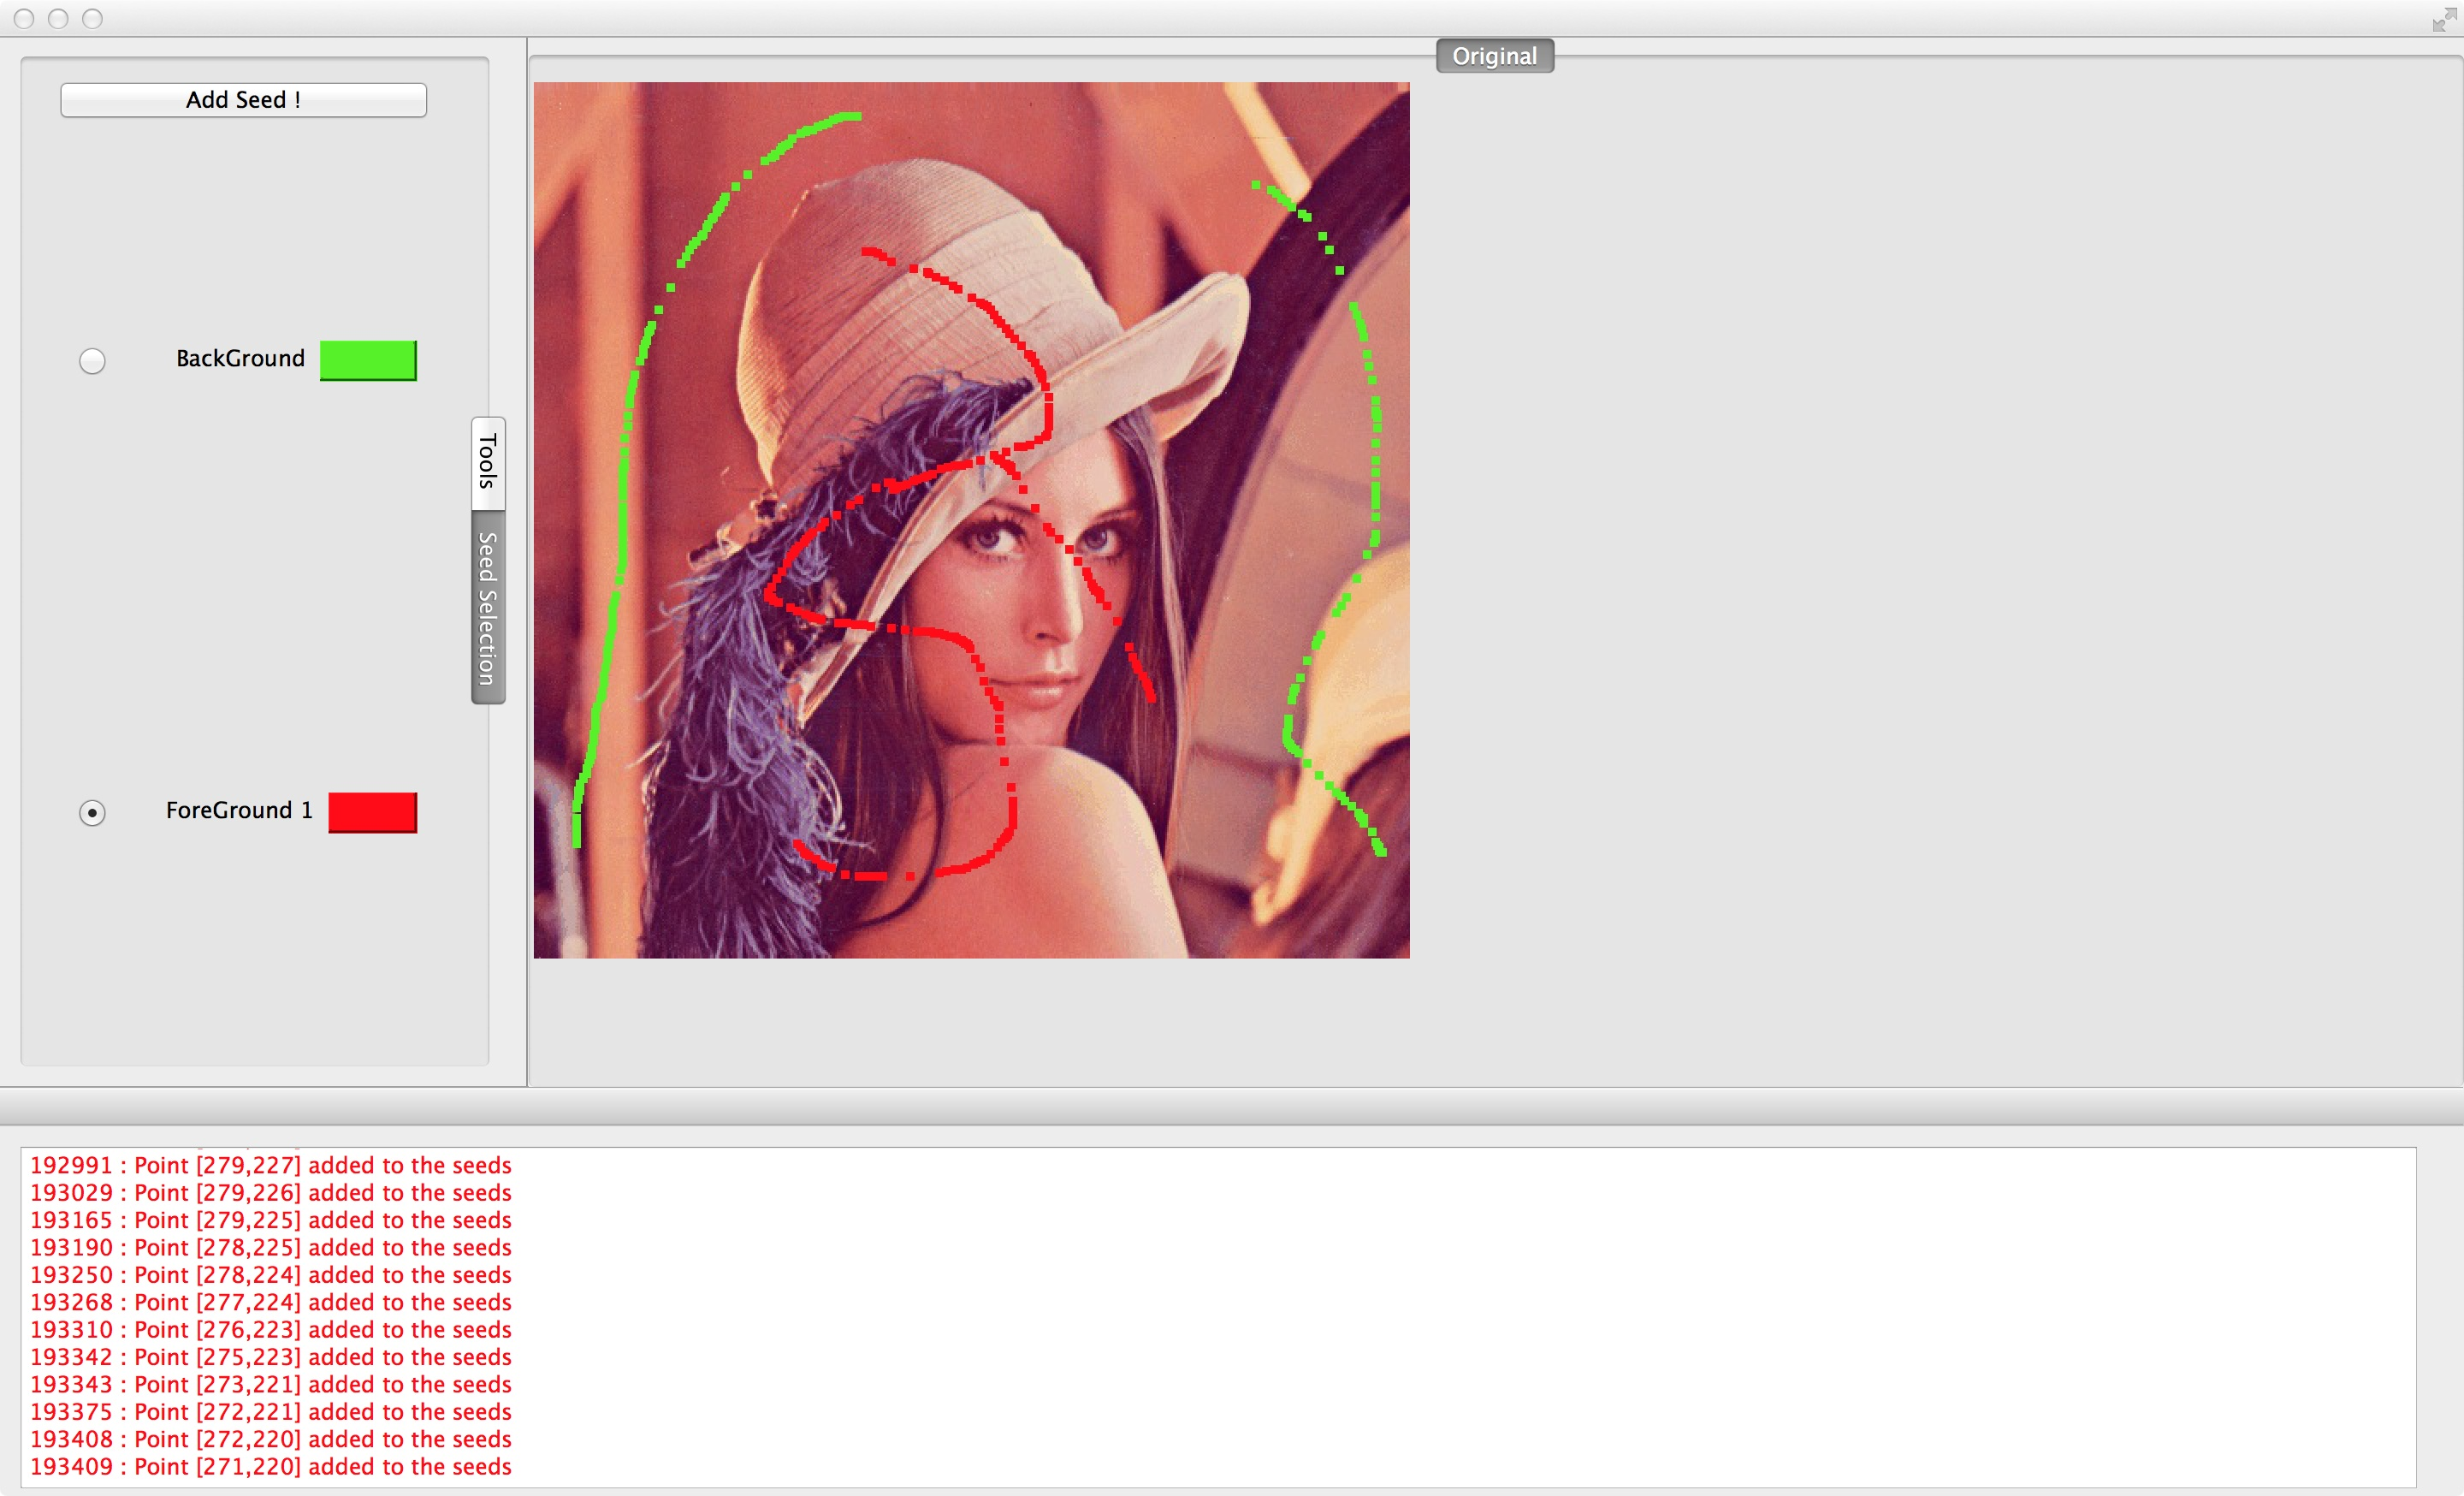
\includegraphics[width=2.4in]{figures/gui_3.jpg}}
  \caption{GUI layout.}
  \end{figure}
\end{minipage}
  \end{minipage}

\end{frame}
%%%%%%%%%%%%%%%%%%%%%%%%%%%%%%%%%%%%%%%%%%%
\subsection{GTest and CMake}
\begin{frame} {System implementation}{GTest and CMake}
GTest:
\begin{itemize}
\item Google Test is an unit testing library. It is available in some languages. We used it for the C++ programming language
\end{itemize}
\vspace{-0.25cm}
\begin{figure}
  \centering
  \subfloat{
\includegraphics[width=0.5in]{figures/testImage.jpg}}
  \caption{Test image for GTest ($9\times 7$ pixels).}
\end{figure}


%\vspace{0.5cm}
CMake:
\begin{itemize}
\item CMake is a cross platform that allows the building of a directory tree outside the source tree
\end{itemize}

\end{frame}
%%%%%%%%%%%%%%%%%%%%%%%%%%%%%%%%%%%%%%%%%%%%%%%
%%%
%%%
%%%%%%%%%%%%%%%%%%%%%%%%%%%%%%%%%%%%%%%%%%%%%
\section{Additional features}
\subsection{Speed vs accuracy}
\begin{frame} {Additional features}{Speed vs accuracy}
  \begin{itemize}
	\item Linear system proposed in Casaca et al.:
\end{itemize}

  \begin{equation}
  (I_{s} + L^{2})x = b
  \end{equation}

\begin{figure}[H]
  \centering
  \subfloat[]{
\includegraphics[width=0.6in]{figures/oriL.jpg}}
  \qquad
  \qquad
    \subfloat[]{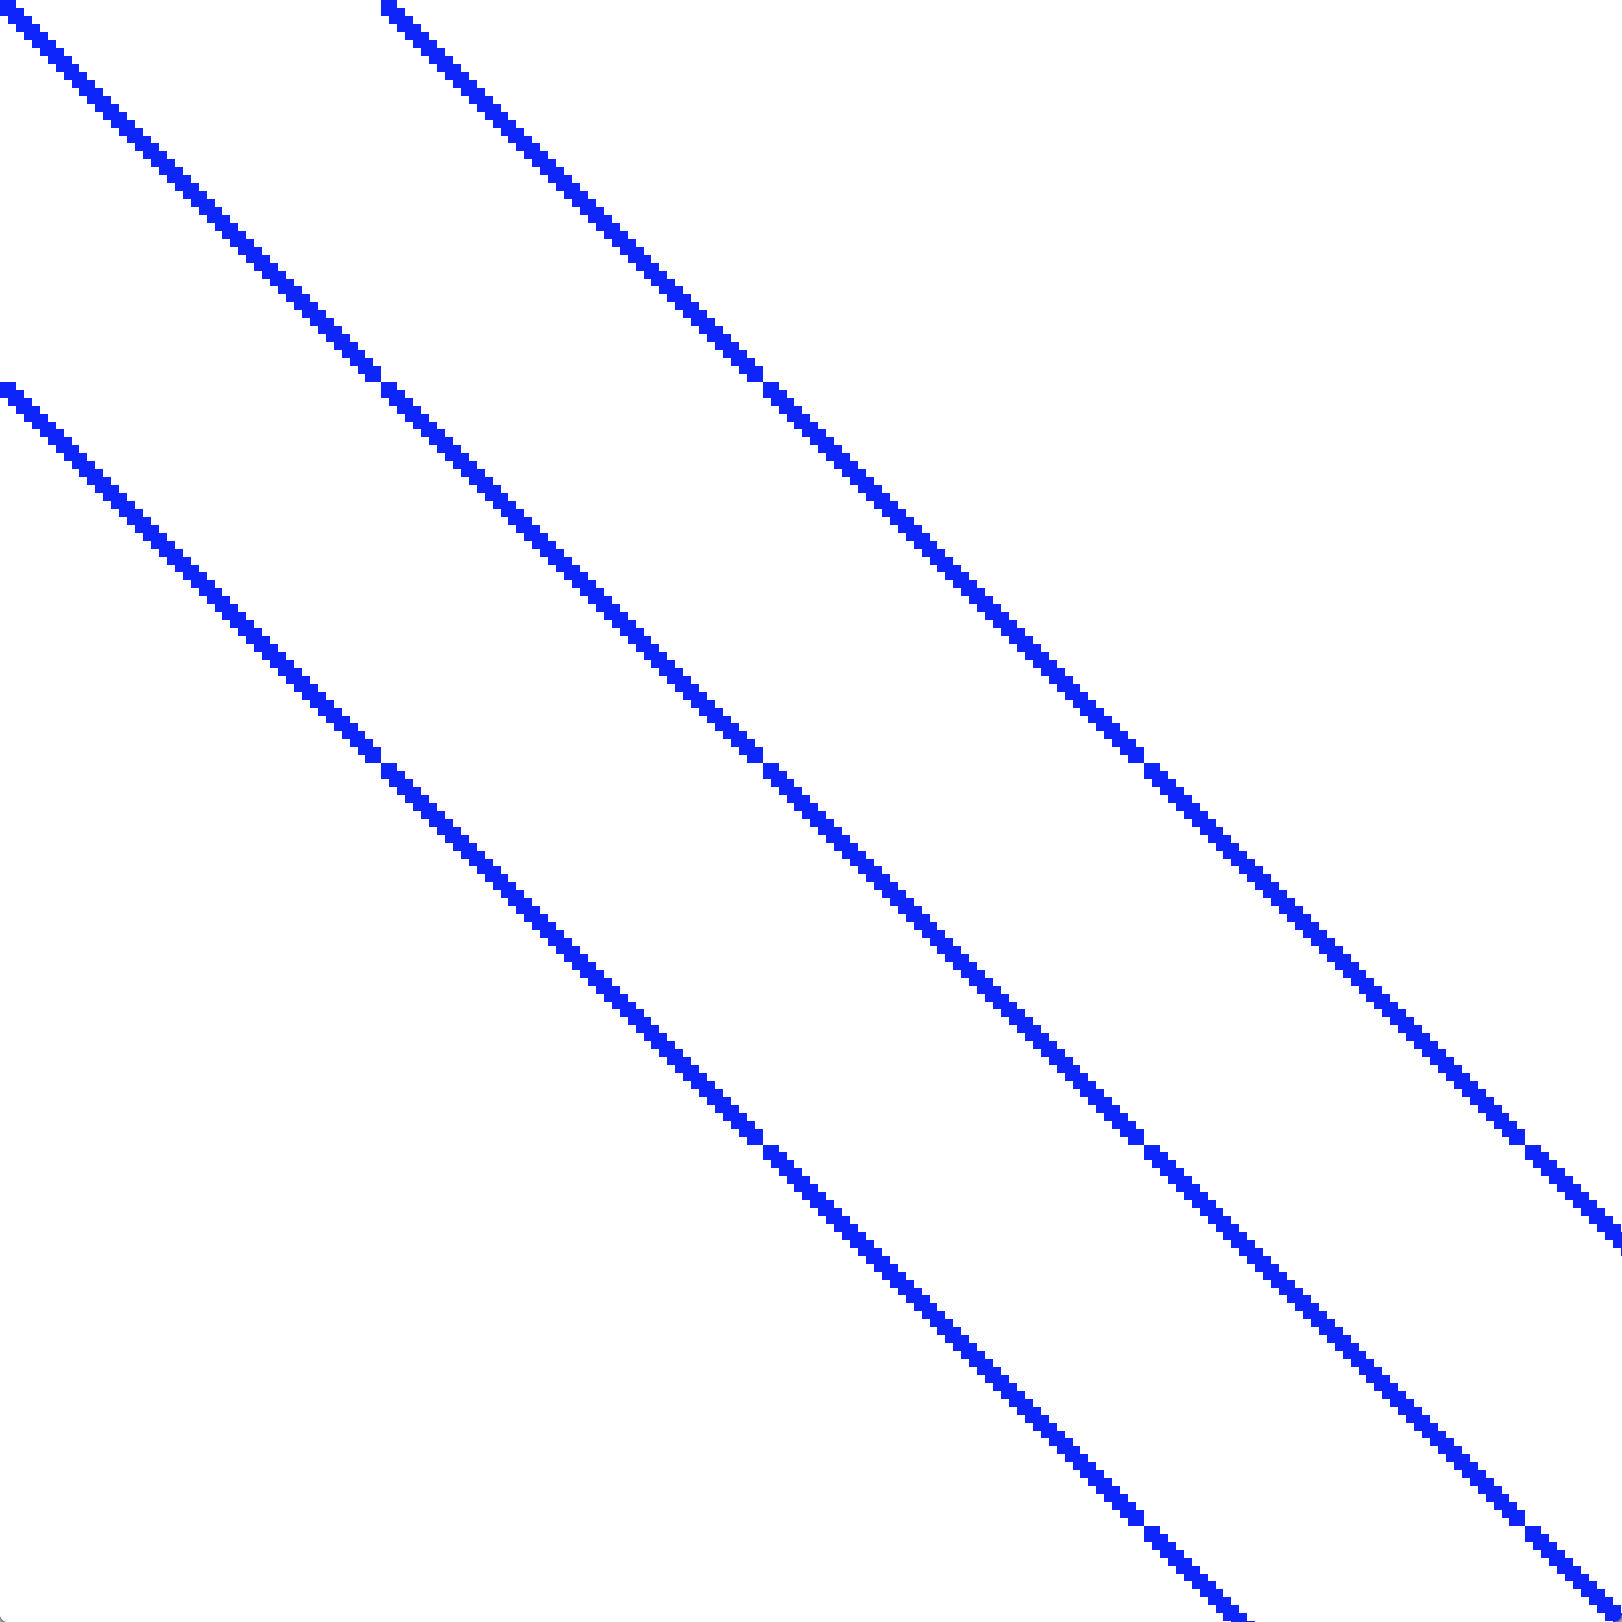
\includegraphics[width=0.6in]{figures/patchL.jpg}}
  \end{figure}
\begin{figure}[H]
  \centering
  \subfloat[]{
\includegraphics[width=0.6in]{figures/oriL2.jpg}}
  \qquad
  \qquad
    \subfloat[]{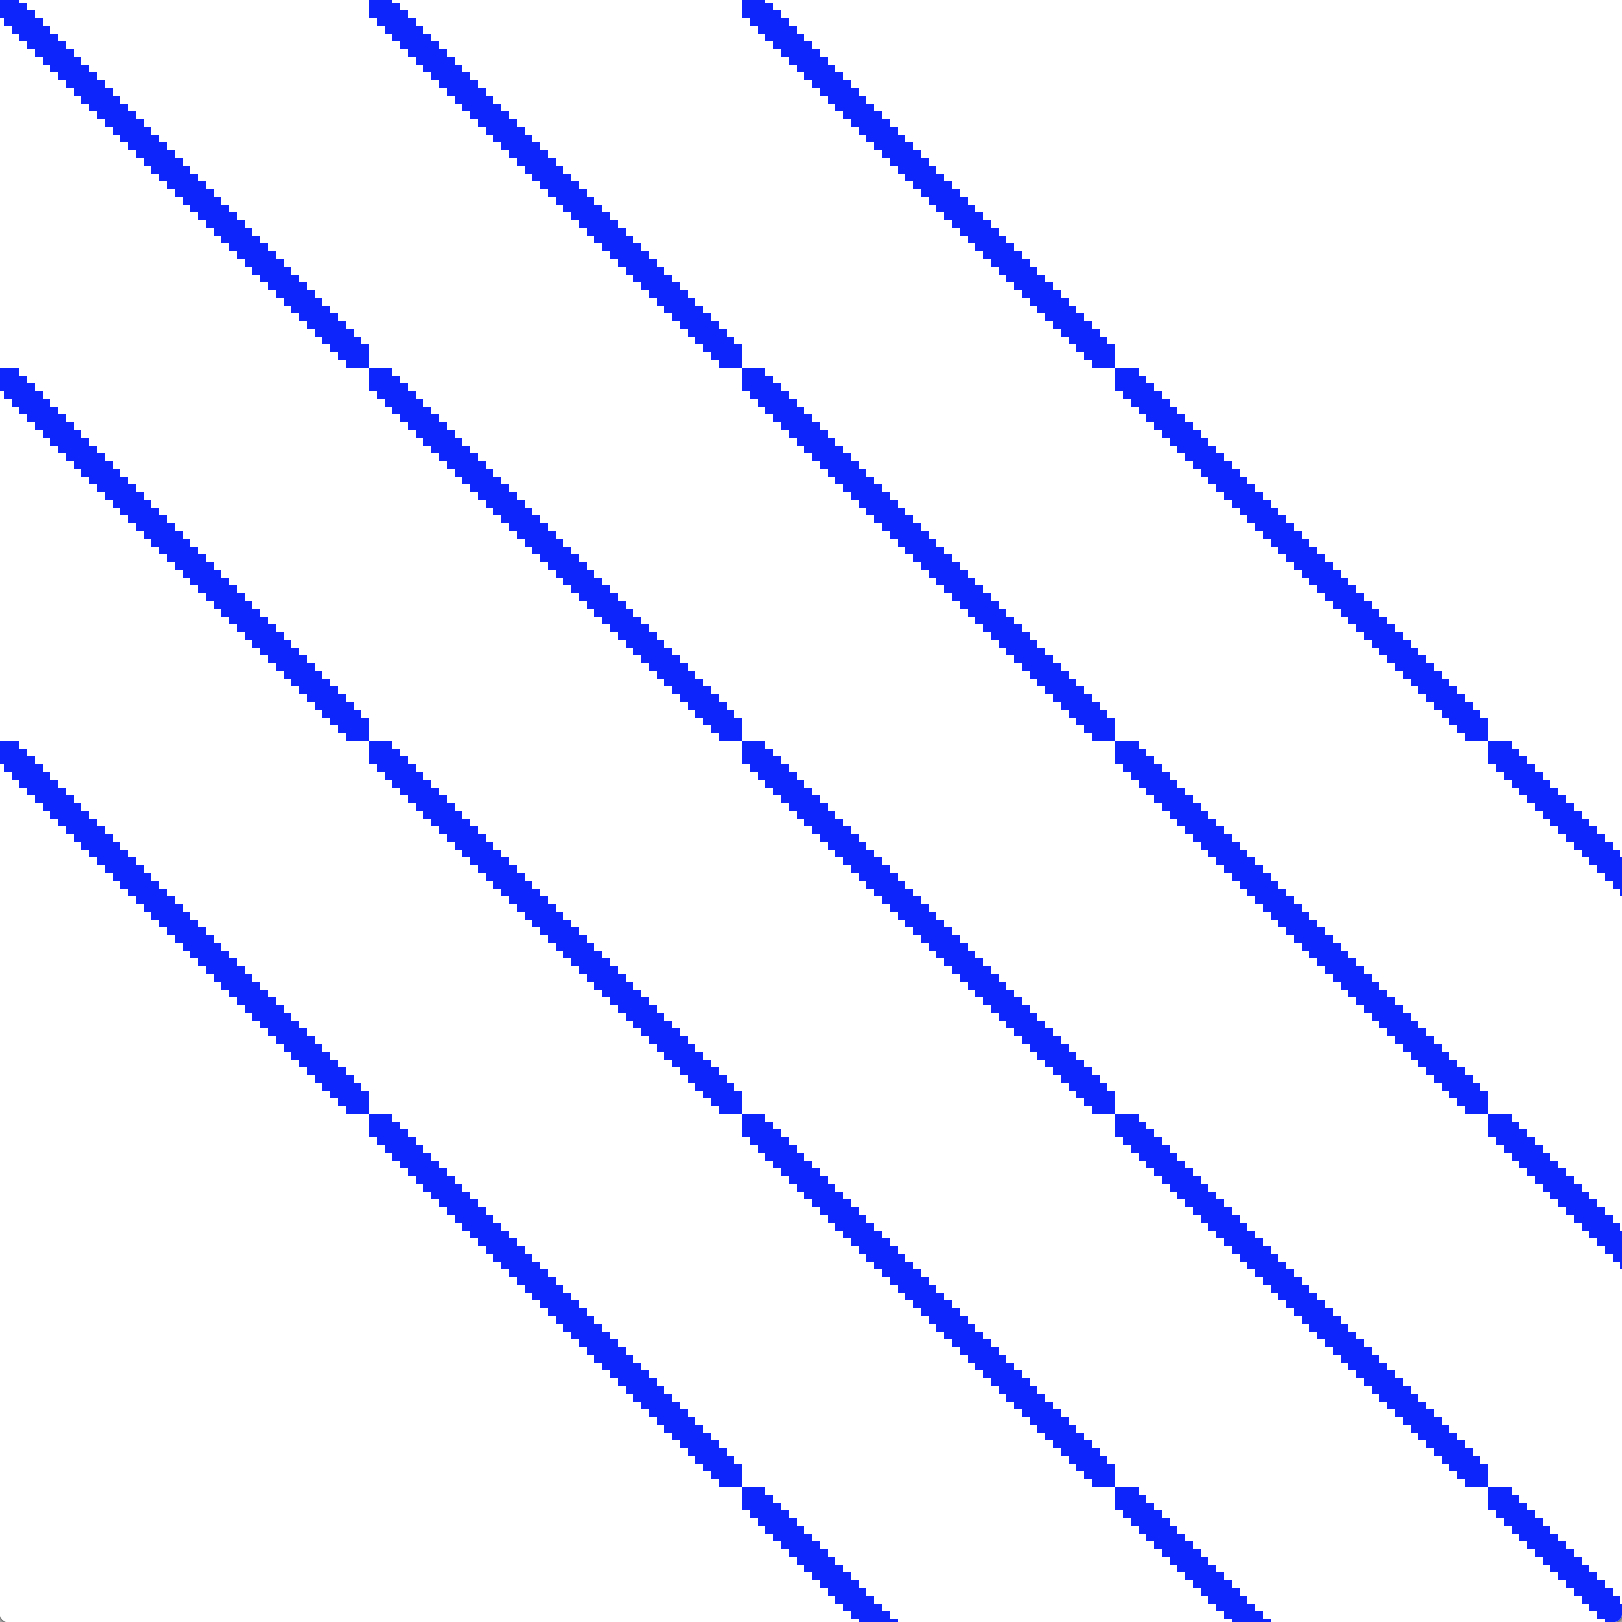
\includegraphics[width=0.6in]{figures/patchL2.jpg}}
    \caption{First row: sparsity of $L$. Second row: sparsity of $L^2$.}
  \end{figure}

\end{frame}
%%%%%%%%%%%%%%%%%%%%%%%%%%%%%%%%%%%%%%%%%%%%
\subsection{Multiple-regions segmentation}
\begin{frame} {Additional features}{Multiple-regions segmentation}
\begin{itemize}
\item On the research paper, in order to achieve multiple segmentation they treat the linear system equation as an extension of solving N linear systems.

\begin{equation}
    (I_{s} + L^{2})x^{(j)} = b^{(j)}
    \end{equation}
    
  \vspace{0.4cm}
 \item No need to compute the matrices $I_s$ and $L$ for each iteration.
 \item The vector $b$ has to be redefined for each segmentation $j$
\end{itemize}
\end{frame}
%%%%%%%%%%%%%%%%%%%%%%%%%%%%%%%%%%%%%%%%%%%%
%%%
%%%
%%%%%%%%%%%%%%%%%%%%%%%%%%%%%%%%%%%%%%%%%%%%
\section{Results and evaluation}
\subsection{Databases}
\begin{frame}{Results and evaluation}{Databases}
\begin{itemize}
	\item Grabcut database
    \item Berkeley Image Segmentation Benchmark Database
\end{itemize}
\vspace{-0.1cm}
\begin{figure}[H]
  \centering
  \subfloat[]{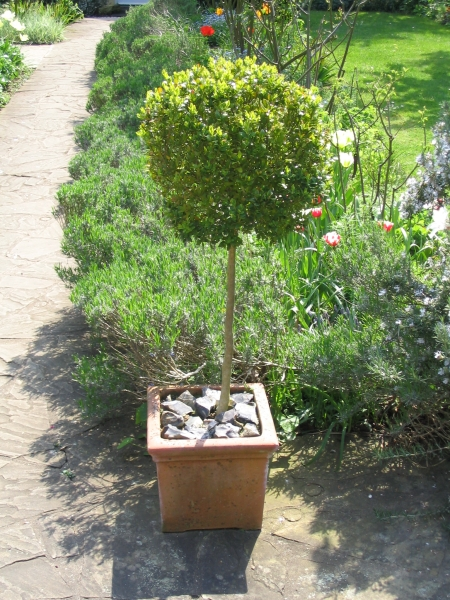
\includegraphics[width=0.65in]{figures/bush.jpg}}
  \qquad
  \subfloat[]{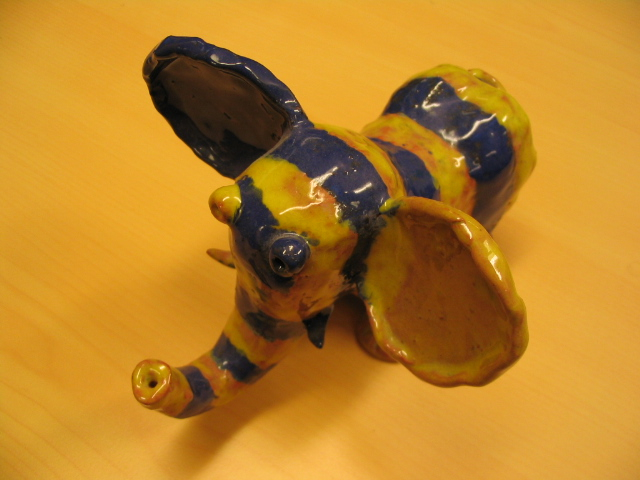
\includegraphics[width=0.65in]{figures/ceramic.jpg}}
  \qquad
  \subfloat[]{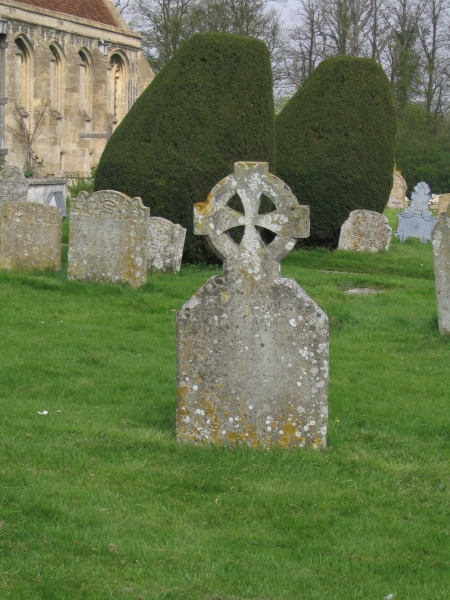
\includegraphics[width=0.65in]{figures/grave.jpg}}
\end{figure}
\vspace{-0.5cm}
\begin{figure}[H]
  \centering
  \subfloat[]{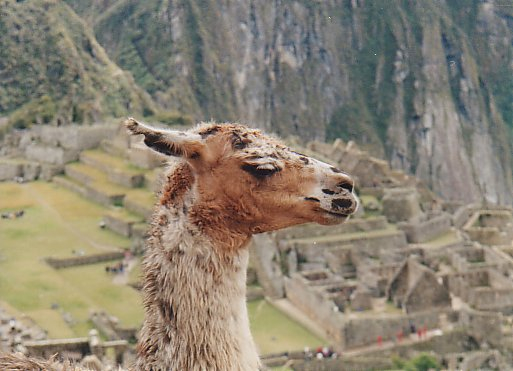
\includegraphics[width=0.65in]{figures/llama.jpg}}
  \qquad
  \subfloat[]{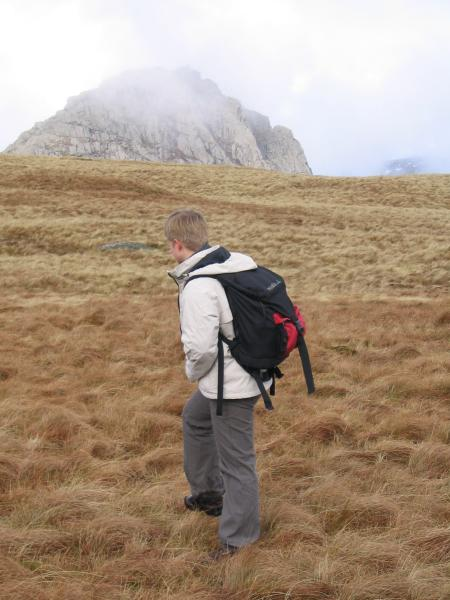
\includegraphics[width=0.65in]{figures/person.jpg}}
  \qquad
  \subfloat[]{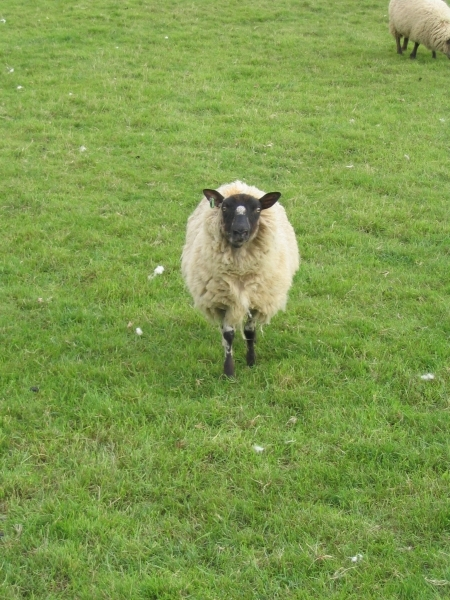
\includegraphics[width=0.65in]{figures/sheep.jpg}}
  \caption{a) bunch. b) ceramic. c) grave. d) llama. e) person. f) sheep.}
\end{figure}

\end{frame}
%%%%%%%%%%%%%%%%%%%%%%%%%%%%%%%%%%%%%%%%%%%%
%%%
%%%
%%%%%%%%%%%%%%%%%%%%%%%%%%%%%%%%%%%%%%%%%%%%
\subsection{Results}
\begin{frame}{Results and evaluation}{Results}

\begin{figure}[H]
  \centering
  \subfloat[]{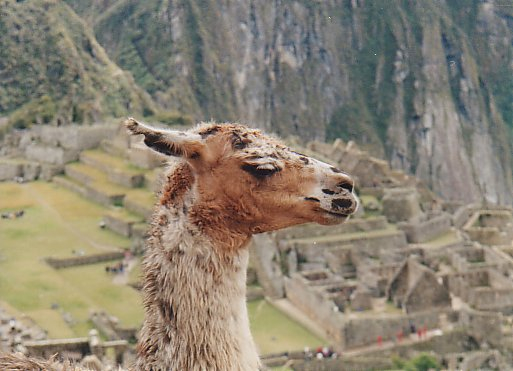
\includegraphics[width=1.05in]{figures/llama.jpg}}
  \quad
  \subfloat[]{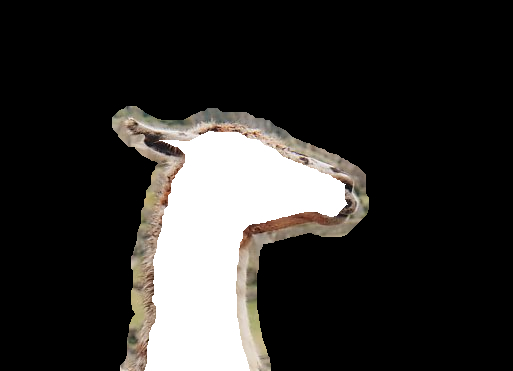
\includegraphics[width=1.05in]{figures/llama_seeds.jpg}}
  \quad
  \subfloat[]{
\includegraphics[width=1.05in]{figures/llama_groundtruth.jpg}}
  \end{figure}
  \vspace{-0.5cm}
  \begin{figure}[H]
  \centering
  \subfloat[]{
\includegraphics[width=1.05in]{figures/llama_L2.jpg}}
  \quad
  \subfloat[]{
\includegraphics[width=1.05in]{figures/llama_L.jpg}}
  \caption{a) original image. b) the tri-map seeds. c) ground-truth. d) obtained result considering L2. e) obtained result considering L.}
  \end{figure}

\end{frame}
%%%%%%%%%%%%%%%%%%%%%%%%%%%%%%%%%%%%%%%%%%%%
%%%
%%%
%%%%%%%%%%%%%%%%%%%%%%%%%%%%%%%%%%%%%%%%%%%%
\subsection{Benchmarking}
\begin{frame}{Results and evaluation}{Benchmarking}
  \tiny{
  \begin{table}[H]
    \renewcommand{\arraystretch}{1.5}
    \caption{Region quality metrics of the six studied images. Evaluation done considering the two studied approaches.}
    \begin{center}

        \begin{tabular}{| >{\centering\arraybackslash\bfseries}m{0.5in} | >{\centering\arraybackslash}m{0.6in} | >{\centering\arraybackslash}m{0.5in} | >{\centering\arraybackslash}m{0.5in} | >{\centering\arraybackslash}m{0.5in} |} \hline
         \textbf{Image} & \textbf{Approach} & \textbf{RI} & \textbf{GCE} & \textbf{VoI} \\ \hline
         \multirow{2}{*}{Bush} & $L^{2}$ & \textbf{0.9441} & \textbf{0.0534} & \textbf{0.4010} \\
         & L & 0.9310 & 0.0665 & 0.4662 \\ \hline
         \multirow{2}{*}{Ceramic} & $L^{2}$ & \textbf{0.9817} & \textbf{0.0117} & \textbf{0.1677} \\
         & L & 0.9796 & 0.0137 & 0.1837 \\ \hline
         \multirow{2}{*}{Grave} & $L^{2}$ & \textbf{0.9840} & \textbf{0.0128} & \textbf{0.1432} \\
         & L & 0.9820 & 0.0144 & 0.1558 \\ \hline
            \multirow{2}{*}{Llama} & $L^{2}$ & \textbf{0.9747} & \textbf{0.0240} & \textbf{0.1781} \\
         & L & 0.9729 & 0.0255 & 0.1857 \\ \hline
         \multirow{2}{*}{Person} & $L^{2}$ & 0.9864 & 0.0097 & 0.1172 \\
         & L & \textbf{0.9868} & \textbf{0.0094} & \textbf{0.1151} \\ \hline
         \multirow{2}{*}{Sheep} & $L^{2}$ & \textbf{0.9900} & \textbf{0.0072} & \textbf{0.0852} \\
         & L & 0.9899 & 0.0073 & 0.0857 \\ \hline
     \end{tabular}
  \label{tb:gantt2}
	\end{center}
  \end{table}
 }

\end{frame}
%%%%%%%%%%%%%%%%%%%%%%%%%%%%%%%%%%%%%%%%%%%
%%%
%%%
%%%%%%%%%%%%%%%%%%%%%%%%%%%%%%%%%%%%%%%%%%%%
\subsection{Accuracy vs speed}
\begin{frame}{Results and evaluation}{Accuracy vs speed}

\begin{figure}[H]
    \centering
    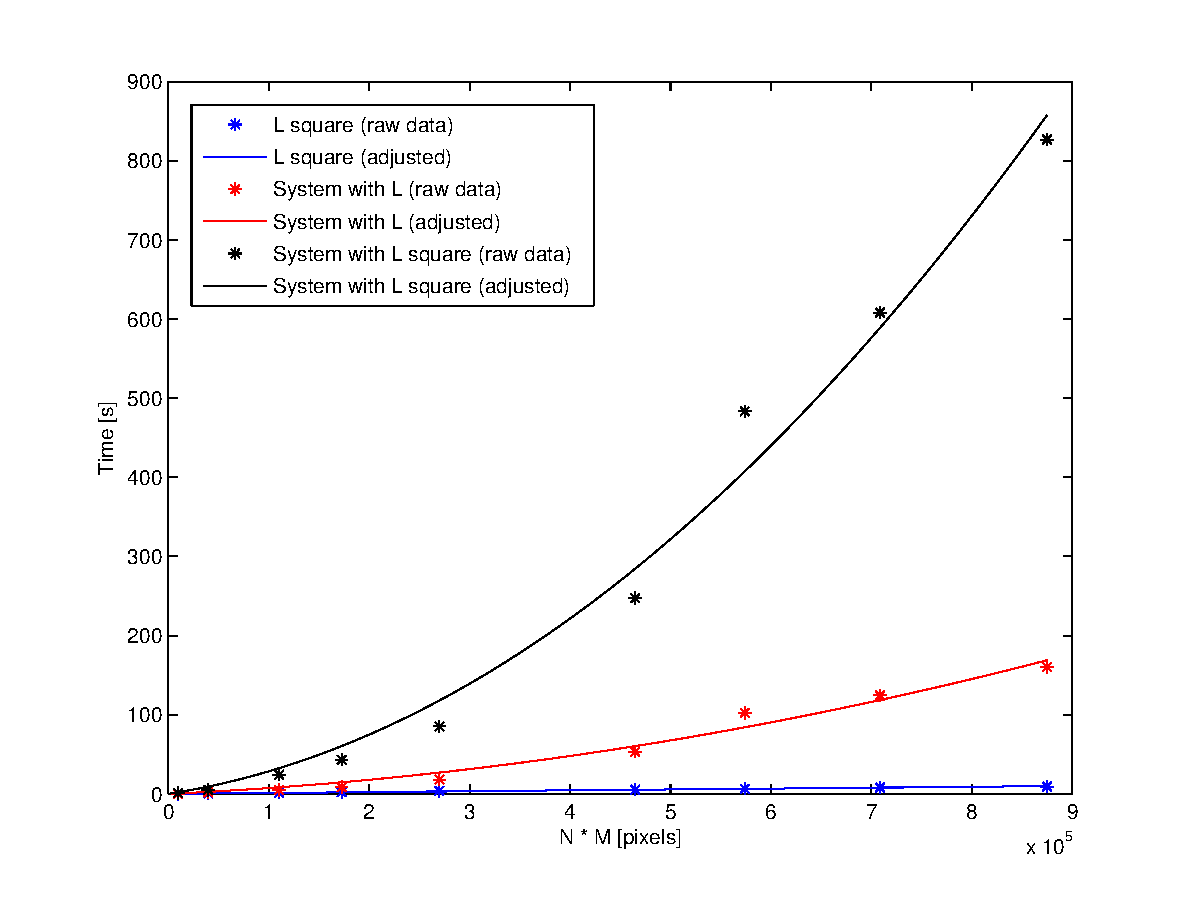
\includegraphics[trim = 9mm 7mm 9mm 10mm, clip, width=6.5cm]{figures/x_LL2_time.eps}
    \caption{Time spent on computing $L^{2}$, on solving the system with L and on solving the system with $L^{2}$ regarding the number of pixels in the image.}
    \label{fig:time_L_vs_L2}
\end{figure}

\end{frame}
%%%%%%%%%%%%%%%%%%%%%%%%%%%%%%%%%%%%%%%%%%%%
%%%
%%%
%%%%%%%%%%%%%%%%%%%%%%%%%%%%%%%%%%%%%%
\subsection{Multi-region segmentation}
\begin{frame}{Results and evaluation}{Multi-region segmentation}

\begin{figure}[H]
  \centering
  \subfloat[]{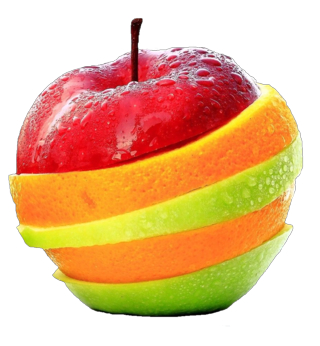
\includegraphics[width=1.15in]{figures/0_apple.jpg}}
  \qquad
  \qquad
  \subfloat[]{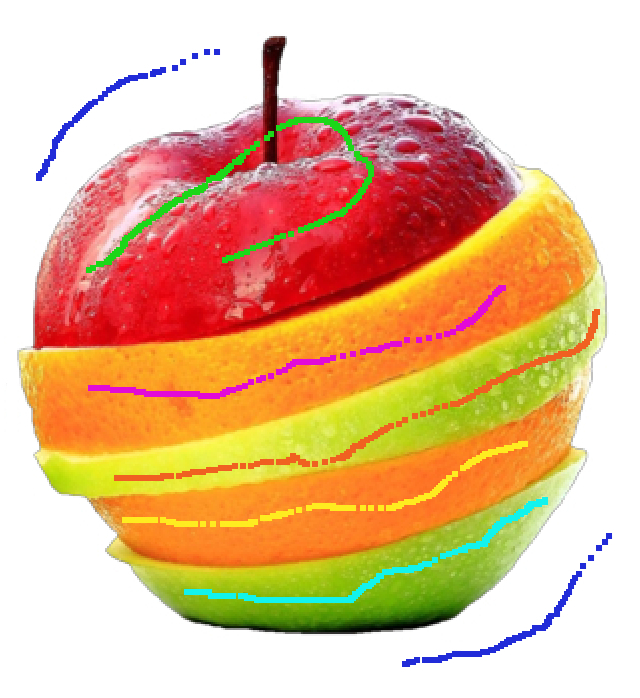
\includegraphics[width=1.15in]{figures/0_seeds.jpg}}
  \caption{a) original image. b) manually selected seeds for multiple-region segmentation.}
\end{figure}

\end{frame}
%%%%%%%%%%%%%%%%%%%%%%%%%%%%%%%%%%%%%%%%%%%%
\begin{frame}{Results and evaluation}{Multi-region segmentation}

\begin{figure}[H]
  \centering
  \subfloat[]{
\includegraphics[width=0.6in]{figures/1_mask.jpg}}
  \qquad
  \subfloat[]{
\includegraphics[width=0.6in]{figures/2_mask.jpg}}
  \qquad
  \subfloat[]{
\includegraphics[width=0.6in]{figures/3_mask.jpg}}
  \qquad
  \subfloat[]{
\includegraphics[width=0.6in]{figures/4_mask.jpg}}
  \qquad
  \subfloat[]{
\includegraphics[width=0.6in]{figures/5_mask.jpg}}
\end{figure}
\vspace{-0.5cm}
\begin{figure}[H]
  \centering
  \subfloat[]{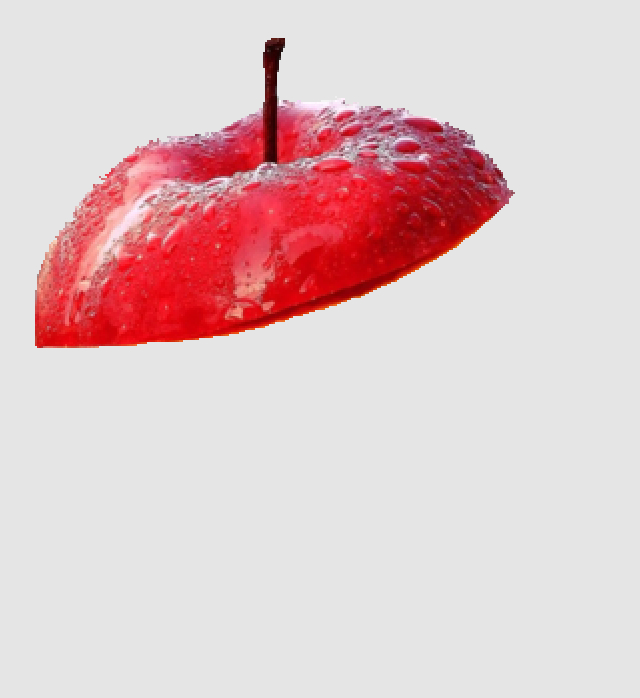
\includegraphics[width=0.6in]{figures/1.jpg}}
  \qquad
  \subfloat[]{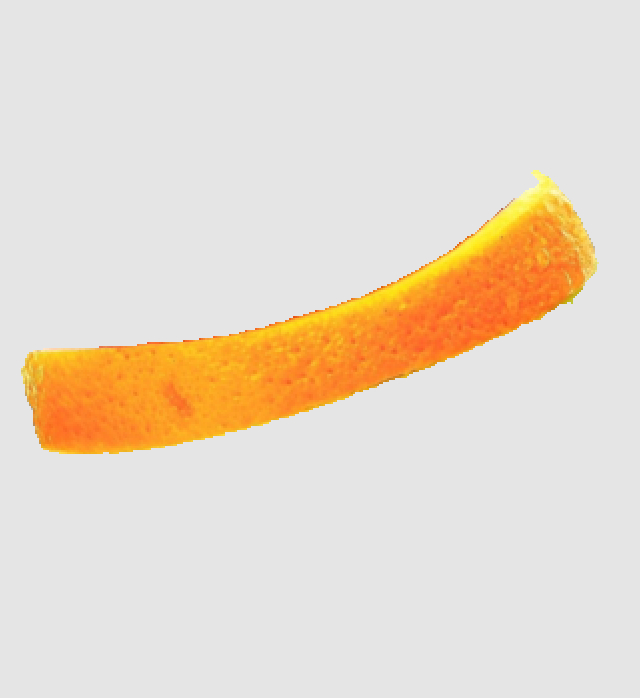
\includegraphics[width=0.6in]{figures/2.jpg}}
  \qquad
  \subfloat[]{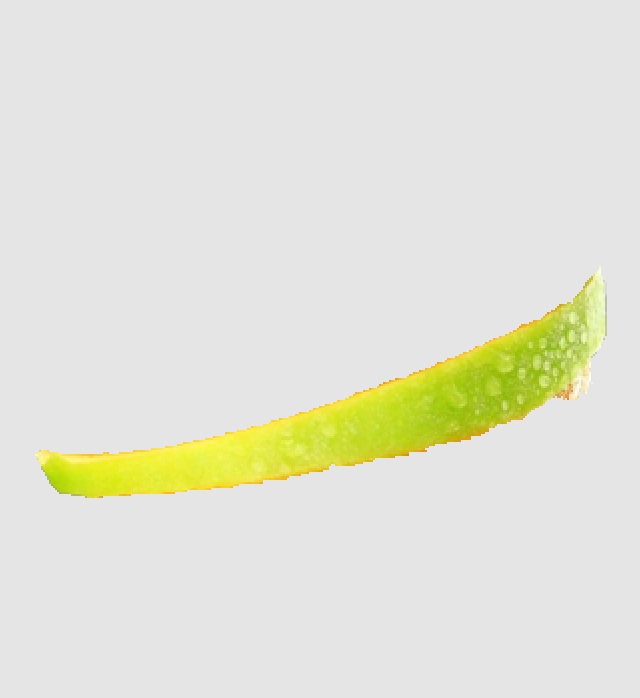
\includegraphics[width=0.6in]{figures/3.jpg}}
  \qquad
  \subfloat[]{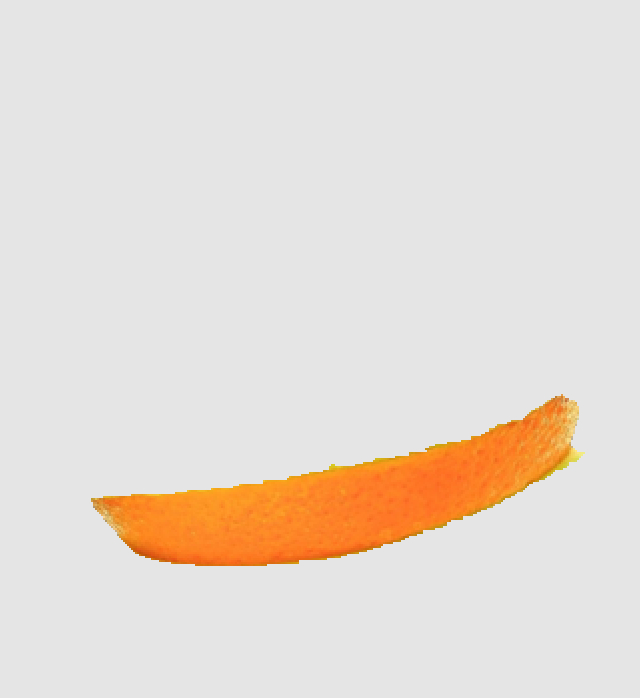
\includegraphics[width=0.6in]{figures/4.jpg}}
  \qquad
  \subfloat[]{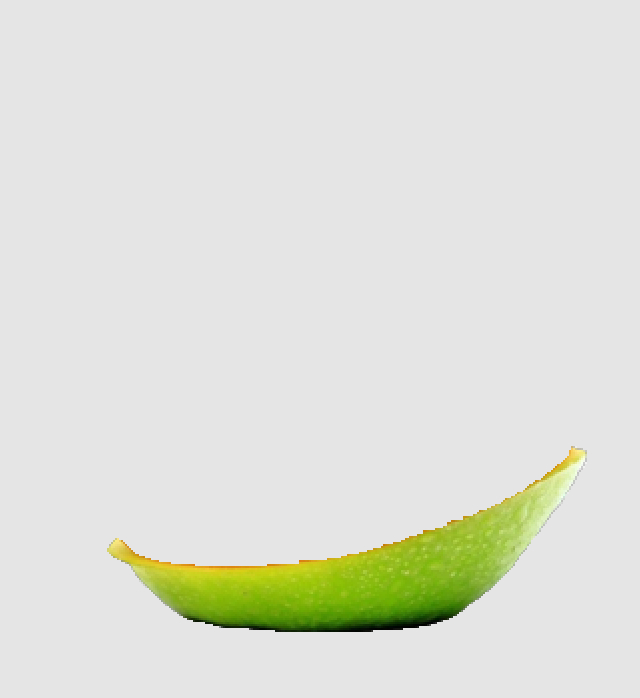
\includegraphics[width=0.6in]{figures/5.jpg}}
  \caption{First row: computed masks. Second row: results after applying the masks.}
\end{figure}

\end{frame}
%%%%%%%%%%%%%%%%%%%%%%%%%%%%%%%%%%%%%%%%%%%%
%%%
%%%
%%%%%%%%%%%%%%%%%%%%%%%%%%%%%%%%%%%%%%%%%%%%
\subsection{DEMO}
\begin{frame}{DEMO}
\begin{figure}[H]
    \centering
    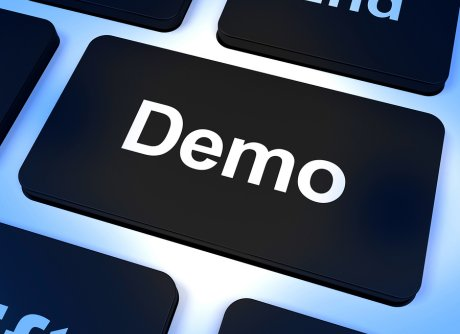
\includegraphics[width=9cm]{figures/demo.jpg}
\end{figure}
\end{frame} 
%%%%%%%%%%%%%%%%%%%%%%%%%%%%%%%%%%%%%%%%%%%%%%%
%%%
%%%%%%%%%%%%%%%%%%%%%%%%%%%%%%%%%%%%%%%%%%%%
\section{Final remarks and future works}
\begin{frame}{Final remarks and future works}
\begin{itemize}
  \item Importance of project management
  \item Open source code
  \item Different method to be studied
  \item Further improvements: real time segmentation
\end{itemize}

\begin{figure}
  \centering
  \subfloat{
\includegraphics[width=1.5in]{figures/cuda.JPG}}
  \caption{Nvidia - Cuda.}
  \end{figure}
  
\end{frame}
%%%% %%%% %%%% %%%% %%%% %%%% %%%% %%%% %%%% %%%% 
%%%% %%%% %%%% %%%% %%%% %%%% %%%% %%%% %%%% %%%% 
%%%% %%%% %%%% %%%% %%%% %%%% %%%% %%%% %%%% %%%% 
\section{Bibliography}
\begin{frame}{Bibliography}
	\begin{itemize}
    \item Linda G. Shapiro and George C. Stockman. \textit{Computer Vision}. Prentice-Hall, ISBN 0-13-030796-3. New Jersey. 2001.
    \item A diffusion approach to seeded image segmentation. Computer Vision and Pattern Recognition (CVPR). June 2010.
    \item Casaca W.,Nonato LG, and Taubin G, \textit{Laplacian Coordinates for Seeded Image Segmentation}. 384-391. June 2014.
    \item C. Rother, V. Kolmogorov, and A. Blake. A database of human segmented natural images and its application to evaluating segmentation algorithms and measuring ecological statistics. Volume 2, pages 416–423. July 2001.
    \item V. Kolmogorov C. Rother and A. Blake. Grabcut: Interactive foreground extraction using iterated graph cuts. ACM
Trans. Graph. (SIGGRAPH 04).
    \end{itemize}
  \end{frame}
%%%%%%%%%%%%%%%%%%%%%%%%%%%%%%%%%%%%%%%%    
\begin{frame}{Bibliography}
	\begin{itemize} 
	\item D. Tal D. Martin, C. Fowlkes and J. Malik. A database
of human segmented natural images and its application to evaluating segmentation algorithms and measuring ecological
statistics. In Proc. 8th Int. Conf. Computer Vision (ICCV).
    \item Google Test. \url{https://en.wikipedia.org/wiki/Google_Test}. 2010. Online accessed: 09-January-2016.
    \item CMake. \url{https://en.wikipedia.org/wiki/CMake}. 2015. Online accessed: 09-January-2016.
    \item Dr. Dobb's Journal of Software Tools, Bibtex-import. 2008-01-15 19:21:54.2000.
    \item Guennebaud and Beno Jacob and others. Eigen v3.2010
	\end{itemize}
\end{frame}

%%%% %%%% %%%% %%%% %%%% %%%% %%%% %%%% %%%% %%%% 
%%%% %%%% %%%% %%%% %%%% %%%% %%%% %%%% %%%% %%%% 
{\1
\begin{frame}[plain,noframenumbering] 
  \titlepage
\end{frame}}
\end{document}